\section{Ergebnisse}
\label{cg:section:ergebnisse}
\rhead{Ergebnisse}

In diesem Abschnitt werden kurz die Ergebnisse der Implementation dargestellt.
Die Implementation wurde mit Python erstellt und ermöglicht eine Konvergenzuntersuchung (Code ist zu finden in \cite{cg:online:code}).
Es zeigte sich, dass die Konvergenzgeschwindigkeit stark von der Konditionierung von $A$ abhängt.
Die Konditionierung wird mit der Konditionszahl $\kappa_A$ gemessen, welche das Verhältnis vom grössten zum kleinsten Eigenwert von $A$ bezeichnet.
Je grösser $\kappa_A$ ist, desto schwerer ist ein Problem zu lösen.
Optimal wäre ein $\kappa_A = 1$, wobei dann die Niveaulininen die Form einer Hyperkugel (Kreis in 2D) annehmen.

Alle nachfolgenden Beispiele lösen ein $N=1000$-dimensionales Problem, was in einer $1000 \times 1000$ Matrix $A$ resultiert.
In Abbildung \ref{cg:abb:slow_conv} sieht man ein Beispiel einer schlechten Konditionierung.
Dabei wird bei etwa $k=200$ Schritten eine Genauigkeit von $10^{-3}$ erreicht.
Abbildung \ref{cg:abb:fast_conv} dagegen zeigt das Verhalten bei sehr guter Konditionierung.
Hier wird bereits nach wenigen Schritten die Genauigkeit von $10^{-3}$ erreicht.
Also haben wir einen starken Einfluss der Konditionierung auf die Konvergenzgeschwindigkeit.
Falls schnelle Konvergenz verlangt wird, kann sich somit eine Präkonditionierung lohnen, welche $\kappa_A$ verbessern würde.

Zum Abschluss zeigt Abbildung \ref{cg:abb:no_conv} was passiert wenn $A$ nicht positiv definit ist.
Das in \ref{cg:subsection:Minimierungsproblem} aufgestellte Minimierungsproblem stimmt dadurch nicht und der CG-Algorithmus scheitert.
Dies äussert sich durch starke Oszillation bei hohem absolutem Fehler.

\begin{figure}	
	\centering
	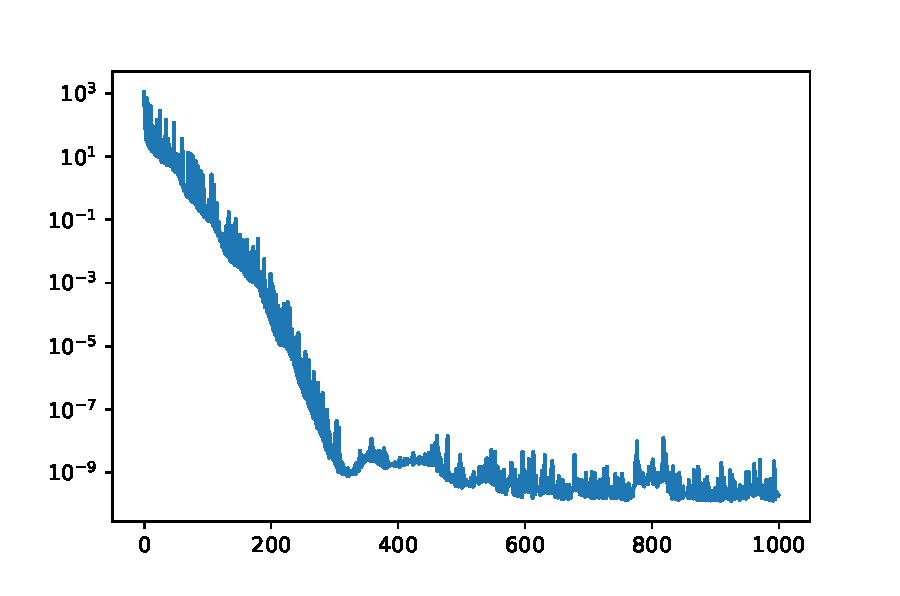
\includegraphics[width=0.8\textwidth]{papers/cg/images/convergence_k_750000}
	\caption{Betrachtung des absoluten Fehlers in Abhängigkeit der Anzahl Schritte bei schlechte Konditionierung ($\kappa_A=750000$).}
	\label{cg:abb:slow_conv}
\end{figure}

\begin{figure}	
	\centering
	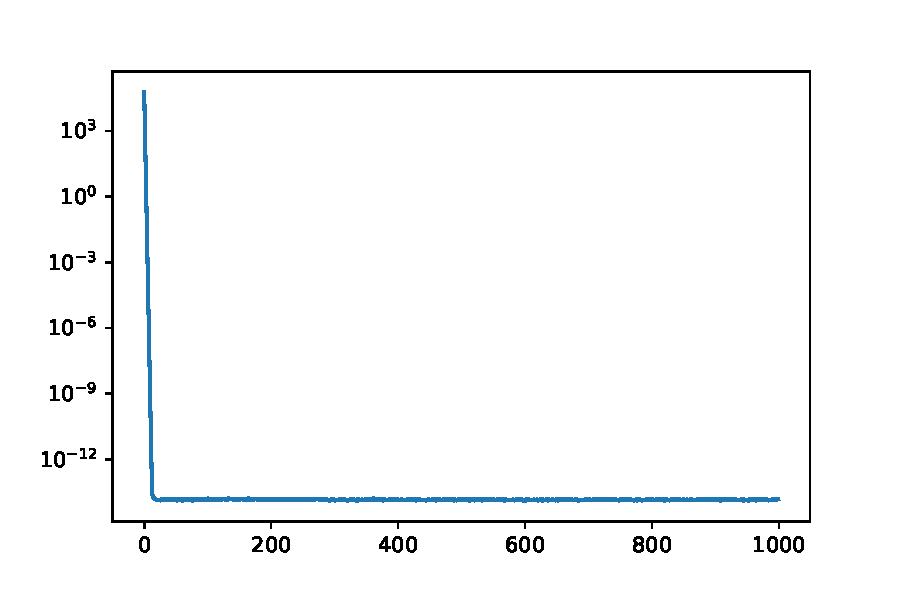
\includegraphics[width=0.8\textwidth]{papers/cg/images/convergence_k_1_1}
	\caption{Betrachtung des absoluten Fehlers in Abhängigkeit der Anzahl Schritte bei guter Konditionierung ($\kappa_A=1.1$).}
	\label{cg:abb:fast_conv}
\end{figure}

\begin{figure}	
	\centering
	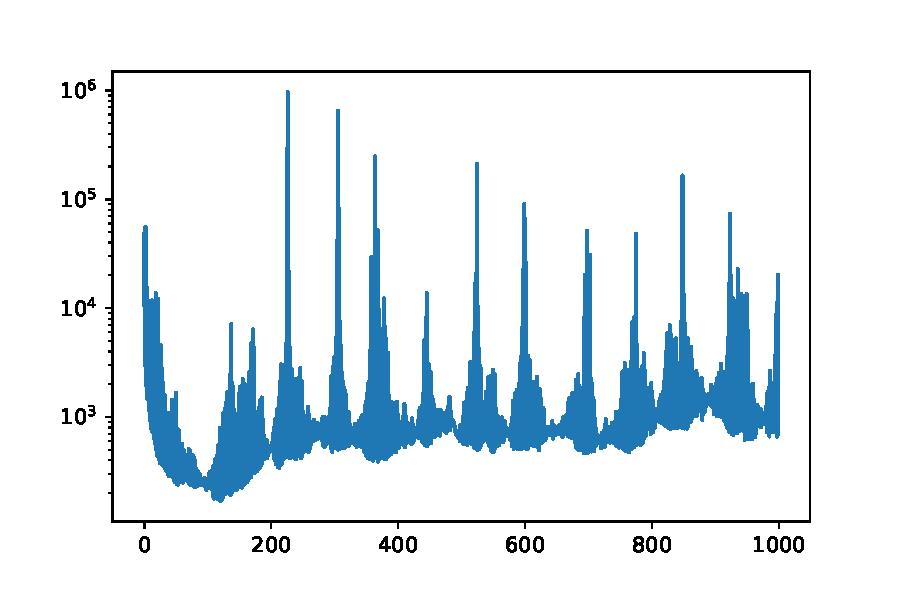
\includegraphics[width=0.8\textwidth]{papers/cg/images/no_convergence}
	\caption{Betrachtung des absoluten Fehlers in Abhängigkeit der Anzahl Schritte falls $A$ nicht positiv definit ist. 
			Es ergibt sich keine Konvergenz.}
	\label{cg:abb:no_conv}
\end{figure}

\subsection{Fazit}
Die hier vorgestellte Methode der konjugierten Gradienten (CG) liefert schnelle, genaue Resultate für grosse lineare Gleichungssysteme.
Besonders interessant ist, dass theoretisch sogar die exakte Lösung gefunden wird (nach $N$ Schritten).
In der Implementation stellt sich dies aufgrund der begrenzten numerischen Genauigkeit natürlich als unmöglich heraus.
Trotzdem ist diese Eigenschaft hilfreich, da es eine fixe Obergrenze für die Anzahl Schritte darstellt.
Falls die Kondition gut ist (was häufig der Fall ist), ist die Konvergenz sehr schnell und es werden deutlich weniger als $N$ Schritte benötigt.